\documentclass[a4paper,12pt]{ujarticle}

% レイアウト
\setlength{\hoffset}{0cm}
\setlength{\oddsidemargin}{-3mm}
\setlength{\evensidemargin}{-3cm}
\setlength{\marginparsep}{0cm}
\setlength{\marginparwidth}{0cm}
\setlength{\textheight}{24.7cm}
\setlength{\textwidth}{17cm}
\setlength{\topmargin}{-45pt}

\renewcommand{\baselinestretch}{1.6}
\renewcommand{\floatpagefraction}{1}
\renewcommand{\topfraction}{1}
\renewcommand{\bottomfraction}{1}
\renewcommand{\textfraction}{0}

% パッケージ
\usepackage[dvipdfmx]{graphicx}
\usepackage{amsmath,amssymb,epsfig}
\usepackage{eucal}
\usepackage{bm}
\usepackage{ascmac}
\usepackage{pifont}
\usepackage{multirow}
\usepackage{enumerate}
\usepackage{cases}
\usepackage{type1cm}
\usepackage{cancel}
\usepackage{url}
\usepackage{color}

% 擬似コード作成用
\usepackage[ruled,vlined]{algorithm2e}
\usepackage{setspace}
%\input{../sty/jdummy.def}

% カウンタの設定
\setcounter{section}{0}
\setcounter{subsection}{0}
\setcounter{subsubsection}{0}
\setcounter{equation}{0}

% キャプションの図をFigに変更
\renewcommand{\figurename}{Fig.}
\renewcommand{\tablename}{Tab.}

% 式番号を式(章番号.番号)に
\makeatletter
\renewcommand{\theequation}{\arabic{section}.\arabic{equation}}
\@addtoreset{equation}{section}
\makeatother

% 表紙
\title{卒業論文\\
汎用フレームと駆動モジュールから構成される\\環境計測ロボットの開発\\
{\large Development of environmental measurement robot consist of general-purpose frame and drive module}
}
\author{\vspace{20mm}\\
指導教員:\ 西田 \hspace{0mm} 健 准教授\\
九州工業大学\ \hspace{0mm} 工学部\\
機械知能工学科\ \hspace{0mm} 知能制御工学コース \\
\vspace{0mm}\\
学籍番号:\ 16104313\\
提出者氏名:\ 山下 \hspace{0mm} 翔\\\vspace{5mm}\\ }
\date{平成29年\ 月\ 日}

% ドキュメントの開始
\begin{document}
% 表紙
\titlepage
\maketitle
\thispagestyle{empty} \newpage
\pagenumbering{roman}
\setcounter{page}{1}
\parindent = 0pt % 字下げOFF

%---------------------------------------
% 概要
\begin{abstract}

\end{abstract}
\thispagestyle{empty}
\newpage
%---------------------------------------
% 目次
\thispagestyle{empty}
\tableofcontents
\newpage
%---------------------------------------
% section 1
\section{序論} \label{intro}
\subsection{研究背景}


\subsection{先行研究}
\ \ 前年度までに開発されたロボットが\label{six_rober}である.森林環境を想定しており,不整地での踏破能力を高めるためにロッカーボギーサスペンションを採用した六輪ロボットである.
3D LiDARを搭載し,森林環境において誤差15cm以下の高精度の三次元地図の作成に成功した.\cite{arita}\\
\ \ しかしながら,この六輪ロボットには複数の問題点が挙げられた.まず,ロボットのサイズが963[mm] $\times$ 962[mm]と森林環境を想定している割には大きい点.さらに重さが約50[kg]あるために取り扱いが非常に不便である点.また,最大の問題として駆動部の構造上,走行困難となる場面が多々あるという点である.\label{problem}

\subsection{研究目的}
\ \ 前述の問題点を考慮し,本研究ではロボットの小型化および構造の簡略化と改善を目的とした.そのための試みとして,ロボットの構造を
\begin{enumerate}
	\item 制御用センターコンピュータ部
	\item 汎用フレーム
	\item 駆動モジュール
\end{enumerate}
の3要素で構成し,各要素について最適化を行った.さらに,森林環境のみならず屋内や平野といった様々な環境に視野を広げるために,2輪・4輪・6輪と組み換え可能なモジュール構造を採用した.
% section 1-1 研究背景
% section 1-2 先行研究
% section 1-3 研究目的
\newpage
%----------------------------------------
% section 2
\section{環境計測ロボット仕様} \label{spec}
\subsection{センターコンピュータ}
\par ロボットの制御用センターコンピュータの構成について以下にまとめる.
\subsubsection{制御用PC}
\par ロボットの制御にはラップトップPCを使用した.CPUはインテル製Core m5(1.10GHz)を搭載しており,OSはUbuntu 14.04LTSを使用した.また,ロボット制御用のミドルウェアとしてROS(Robot Operating System)を使用した.
\subsubsection{モータドライバ}

\par モータドライバはCytron Technologies製 2ch DCブラシモータドライバ MDD10A(Fig.\ref{MDD10A})
を使用した.本製品はPWM信号を入力することにより速度制御を行うことができる.
\par ロジック電圧は5[V]であり,後述のモータコントローラを介してPCから給電される.

\begin{figure}[hb]
	\centering
	\includegraphics[clip,scale=0.08]{./figure/MDD10A.eps}
	\caption{MDD10A}
	\label{MDD10A}
\end{figure}
\newpage
\subsubsection{モータコントローラ}
\par エンコーダパルスカウンタおよびモータコントローラには iXs Research製 超小型USB接続4chモータコントローラ iMCs01(Fig.\ref{iMCs01})を使用した.本製品は最大3組のエンコーダ・DCモータの制御が可能である.また,入力には2相エンコーダ入力信号(4000pps未満),出力はPWM信号・CW/CCWが利用可能である.さらに,USBでPCから直接制御することが可能かつ,内部にPID制御式(\ref{imcs_eq})を持っているためにプログラム上でゲインの設定を行うだけで用意に制御が可能である.
制御出力 u は次式から 1[ms]毎に計算される.

\begin{eqnarray}
	u=A-\frac{K_P}{K_{P_x}}(v_d - v)%-\frac{K_D}{K_{D_x}}(\dot v_d - \dot x)
	-\frac{K_I}{K_{I_v}}\sum_0^t (v_d-v)
\label{imcs_eq}
\end{eqnarray}

このとき,Aはオフセットであり,$K_P・K_I$はそれぞれ比例・積分ゲインである.また,$v_d$は目標速度,$v$は現在値である.\\
\par ただし,本モータコントローラは本来位置制御に特化したものであるので現在値を得る際には,
\begin{equation}
	v = \frac{x_i - x_{i-1}}{t}
\end{equation}
から求める.このとき$x_i$は現在位置, $x_{i-1}$は1ステップ前の位置であり,$t$は1ステップの時間である.

\begin{figure}[hb]
	\centering
	\includegraphics[clip,scale=0.06]{./figure/IMCS01.eps}
	\caption{iMCs01}
	\label{iMCs01}
\end{figure}

\subsubsection{電源}
石川鉄鋼所にきかなければー
%--------------------------------------------------------------------------------------------------
\subsection{汎用フレーム} \label{frame}







%-------------------------------------------------------------------------------------------------- 
\newpage
\subsection{駆動モジュール} \label{module}
\subsubsection{駆動モジュール構成}
\par 駆動モジュールはDCモータ,ロータリエンコーダ,ホイールによって構成されている.概念図と実際に製作した駆動モジュールをFig.\ref{drivingmod}に示す.各部はギアによって伝達されており,モータとエンコーダのギア比は2:1,モータとホイールのギア比は1:2となっている.\\
\par また,\ref{DCmotor}で示すDCモータを使用した際にこのモジュールが出せる最高速は,$0.774$[m/s]である.このとき$D$は車輪の直径である.

\begin{eqnarray}
	Vel_{max}  &=&\frac{rpm}{60sec}\cdot \pi \cdot	D\\ \nonumber
	 &=&\frac{98.5}{60}\cdot \pi \cdot 0.15 = 0.774
\end{eqnarray}

\begin{figure}[ht]
	\centering
	\begin{tabular}{cc}

		\begin{minipage}{0.5\hsize}
		\centering
		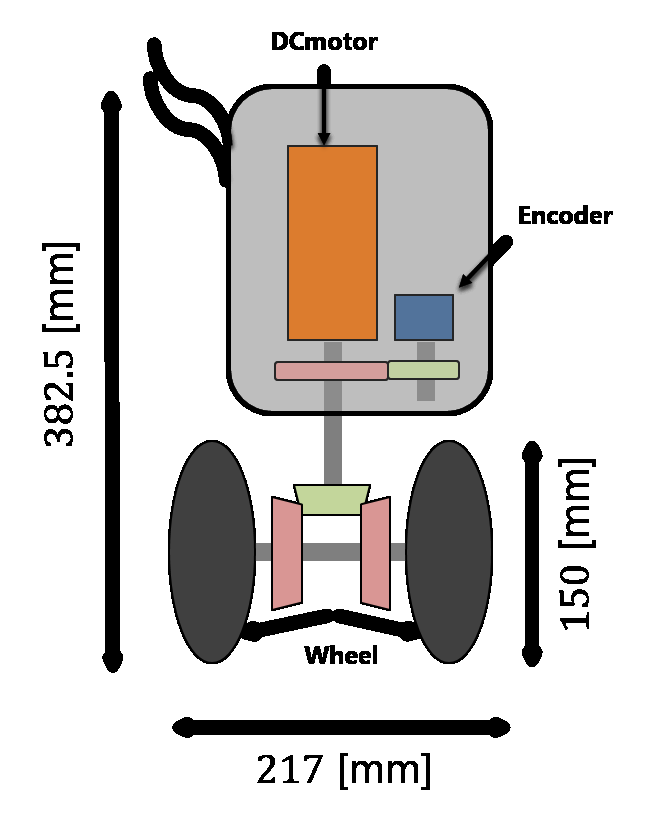
\includegraphics[clip,scale=0.5]{./figure/drivingmod_fig.eps}
		\hspace{1.6cm}
		\caption{概念図}
		\end{minipage}

		\begin{minipage}{0.5\hsize}
		\centering
		\includegraphics[clip,scale=0.06,angle=270]{./figure/driving_mod.eps}
		\hspace{1.6cm}
		\caption{製作した駆動モジュール}
		\end{minipage}

	\end{tabular}	
	\caption{駆動モジュール}
	\label{drivingmod}
\end{figure}
\newpage
\subsubsection{DCモータ}\label{DCmotor}
\par 各モジュールは駆動用としてそれぞれDCモータを搭載している.モータには,シンクエンジニアリング製 TE-38F16-24-64(Fig.\ref{dc-motor})使用した.モータ仕様をTab.\ref{motor_spec}に示す.

\begin{figure}[hb]
	\centering
	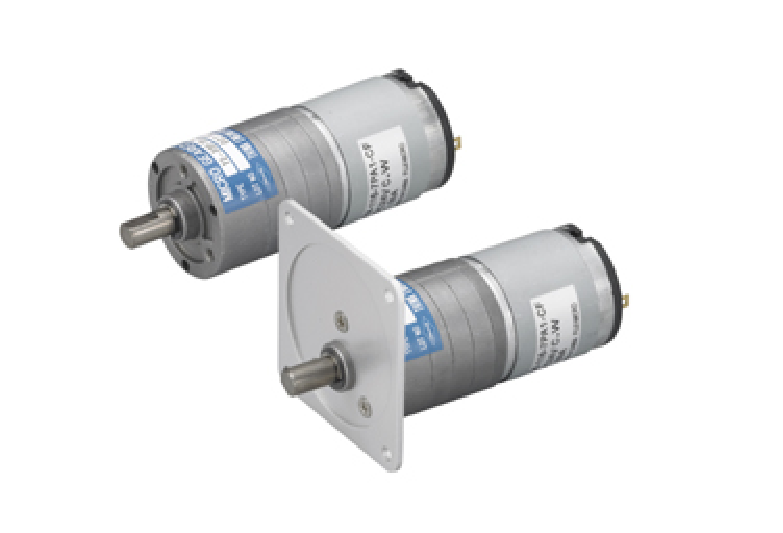
\includegraphics[clip,scale=0.2]{./figure/te-38f16-24-64.eps}
	\caption{DCモータ}
	\label{dc-motor}
\end{figure}

\begin{table}[hb]
	\centering
	\caption{DCモータ仕様}
	\begin{tabular}{|c|c|c|c|c|} \hline
		Rotation speed (rpm) & Torque(mN$\cdot$m) & Current (A) & Length (mm) & Weight (kg)  \\ \hline \hline
		98.5 & 1881.6 & 2.3 & 77.0 & 360.0 \\ \hline
	\end{tabular}
	\label{motor_spec}

\subsubsection{ロータリエンコーダ}
\par 車輪回転速度制御用に,各駆動モジュールにはomron製インクリメンタル型ロータリエンコーダE6A2-CW3E(Fig.\ref{encoder_fig})を搭載している.仕様についてTab.\ref{encoder_spec}にまとめる.


\end{table}
\begin{figure}[hb]
	\centering
	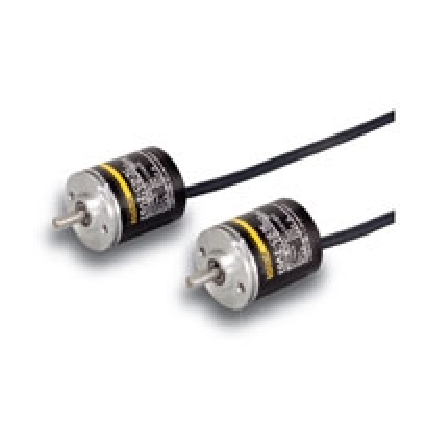
\includegraphics[clip,scale=0.5]{./figure/e6a2-c.eps}
	\caption{インクリメンタル型ロータリエンコーダ}
	\label{encoder_fig}
\end{figure}

\begin{table}[hb]
	\centering
	\caption{ロータリエンコーダ仕様}
	\begin{tabular}{|c|c|c|c|} \hline
		Power-supply (V),(mA) & Output phase & Output type & Maximum speed (rpm) \\ \hline \hline
		5-12,30 & A,B & Voltage & 5000 \\ \hline
	\end{tabular}
	\label{encoder_spec}
\end{table}
\newpage

%--------------------------------------------------------------------------------------------------
\subsection{3DLiDAR} \label{LiDAR}
\par 開発したロボットは環境を計測するための三次元計測センサとして,北陽電機社製3DLiDAR YVT-35LXを搭載している(Fig.\ref{yvt-35lx}).YVT-35LXの主なスペックをTab.\ref{yvt_spec}に示す.


\begin{figure}[hb]
	\centering
	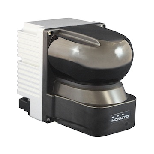
\includegraphics[clip,scale=2.5]{./figure/yvt-35lx.eps}
	\caption{3D LiDAR YVT-35LX}
	\label{yvt-35lx}
\end{figure}

\begin{table}[hb]
	\centering
	\caption{3D LiDAR YVT-35LX 仕様}
	\begin{tabular}{|c|c|} \hline
	& Specification \\ \hline
	Power 				& 10-30 [V](DC) \\ \hline
	Horizontal scan angle	& 210 [deg] \\ \hline
	Horizontal scan speed	& 20 [Hx]	\\ \hline
	Vertical scan angle		& 40 [deg](-5 - 35 [deg]) \\ \hline
	Vertical scan speed		& 1200 [Hz]	\\ \hline
						& 0.3-35 [m]($\-45<\theta < 45 $[deg]) \\
	Sensing distance	& 0.3-20 [m]($\-75 < \theta < -45,45<\theta<75$[deg]) \\
 						& 0.3-10 [m]($\theta< -75,75< \theta$[deg]) \\ \hline
	Accuracy			& $\pm$ 50 [mm](less than15[m]),$\pm$100[mm](than 15[m])\\ \hline
	Points of data		& 2590[points/frame] (20[fps])	\\ \hline
	Interface			& Ethernet(TCP/IP)				\\ \hline
	Weighy				& about 650[g]	\\ \hline
	Size				& 70[mm]$\times$106[mm]$\times$95[mm](W$\times$D$\times$H)\\ \hline
	\end{tabular}
	\label{yvt_spec}
\end{table}

% section 2-1 センターコンピュータ
% section 2-2 汎用フレーム
% section 2-3 駆動モジュール
% section 2-4 3DLiDAR
\newpage
%-----------------------------------------
% section 3
\section{環境地図作成} \label{mapping}
\subsection{マッピング手法}

\subsection{地図生成}
% section 3-1 マッピング手法
% section 3-2 地図生成
\newpage
%-----------------------------------------
% section 4
\section{計測実験} \label{experiment}
\par 製作したロボットについて,駆動モジュール数を変更することで計測環境に適したロボットとなるか,および高精度の三次元地図の生成を行うことができるかを確認するために検証実験を行った.
\subsection{実験内容}
\par 実験は\ref{fields}に示す3つの環境で行った.それぞれ
\begin{itemize}
	\item 室内(平坦な環境)
	\item 砂利道(起伏のある環境)
	\item 森林(不安定かつ障害物のある環境)
\end{itemize}
である.これらに対して,\ref{frame}に示した汎用フレームに2・4・6つの駆動モジュールを組込んだ3種のロボットを用いて比較のための3次元環境計測実験を行った.
また,それぞれは小回りの利く独立二輪機構,走破性と安定性を重視した四輪機構,不整地に対する走破性に重きをおいた六輪ロッカーボギー機構を有する.

\subsection{実験手順}
\par 各実験環境において,各種ロボットを遠隔操作によって走行させ,3次元地図を作成した.その際に,走行・計測完了までのタイム,地図の精度,(検討中)について比較を行う.地図の精度についてはその要因となりうるロボット本体の揺れについても,3DLiDAR(\ref{LiDAR})のIMU機能を用いて検証を行う.


% section 4-1 実験内容
% section 4-2 実験手順
\newpage
%-----------------------------------------
% section 5
\section{実験結果および考察} \label{result}

% section 5-1 結果
% section 5-2 比較・検討
\newpage
%-----------------------------------------
% section 6
\section{結論} \label{conclusion}

%-----------------------------------------
\section*{謝辞} \label{thanks}

\end{document}